%---------------------------------------------------------------------------------------------------
% Tests
%---------------------------------------------------------------------------------------------------
\newpage
%\part{Anfang}
\chapter{Tests}\label{cap:Tests}

When lots of puzzle pieces come together, it is sometimes difficult to see the big picture. The same happens during the software development process. Providing a bugfree application is a big task.
In software development, misfunctioning features are called bugs. They appear in many situations, and it is a tough task to avoid or fix these bugs. Getting close to this goal testing is very important though. Different aspects of testing have to be taken into consideration. Professional companies with a appropriate budget prefer the \textbf{t}est \textbf{d}riven \textbf{d}evelopment (TDD) approach. TDD means that the tests are written before the functions did. There are also different techniques available, unit, integration, and end-to-end tests build the so-called testing pyramid. The test environment is also worth to mention. However, In this study, unit tests were carried out.

\section{Unit Test}
Testing a unit is an encapsulated case. The input is known, something happened within the test method, and the output must be equal to the expectation.
As mentioned in the design chapter during the filter section, the filtering method is a decent unit test case (list. \ref{code:test_map_activity_filter}). 
 
\begin{mdframed}
\lstinputlisting[label={code:test_map_activity_filter} ,caption={Unit testing filter method},captionpos=b, style=MeinStyle, numbers = left]{program/test_map_activity_filter.java}
\end{mdframed}

Starting with the instantiation of the global test variable SUT (System Under Test), one performs the desired method on this SUT variable. Before and after each test, the input gets prepared according to the desired specifications. In this case, before each test, a list of artefacts with four entries gets prepared. The list becomes cleared afterwards. The result depends on the conditions within the test. Searching and handling edge cases leads to a robust result. A convention determines that the name of the test method should give information about the test conditions and the result (fig. \ref{fig:test_as_filter_unit_test}). 

\begin{figure}[H]
    \centering 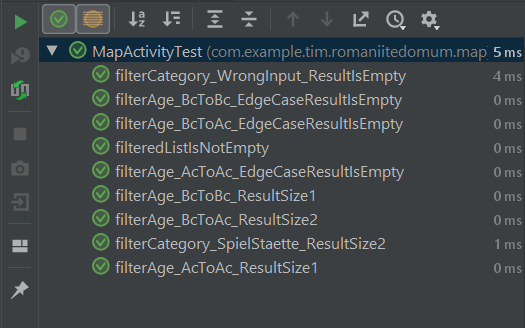
\includegraphics[width=0.8\textwidth]{test/test_as_filter_unit_test.PNG}
    \caption[Successful unit test]{Successful unit test}
    \label{fig:test_as_filter_unit_test}
\end{figure}

Due to a lack of time, the filtering method is the only unit that has been tested.

\section{Test Environment}
Android Studio provides an integrated emulator tool. One can simulate popular mobile devices, like Nexus, Google Pixel, and others (see \ref{fig:testdevice_overview}).

\begin{figure}[H]
    \centering 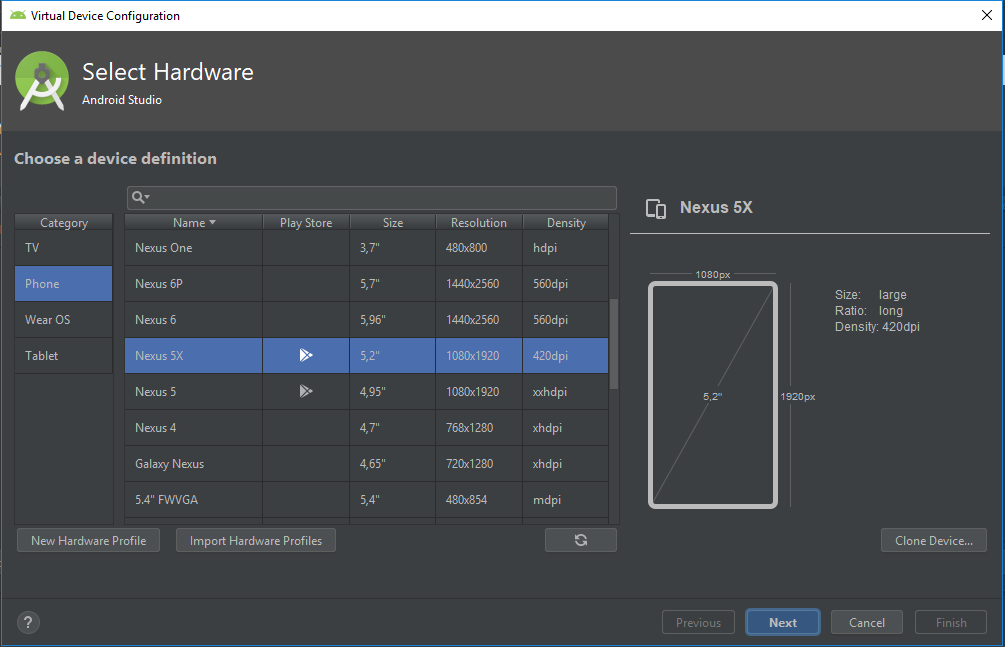
\includegraphics[width=0.8\textwidth]{test/testdevice_overview.PNG}
    \caption[Android Studio emulator overview]{Android Studio emulator overview}
    \label{fig:testdevice_overview}
\end{figure}

Alternatively, one can set up a custom device to fit their demands. There are plenty of tutorials with the topic "how to set up a custom emulator", so an explanation will be out of the scope of this thesis. 
Even though the Android Studio emulator is well done, emulator tests cannot replace real device testing.
User experience goes hand in hand with the haptical behaviour of the app. Therefore the Civitas app was also extensively tested on the developer devices, a \textit{UMIDIGI Z} and a \textit{Huawei P Smart (2019)}. 

An approach to making device testing more pleasant is realized with the VYZOR software. VYZOR acts like a mirror and displays the device on to the computer monitor.  




